\documentclass[12pt,letterpaper]{article}\usepackage[]{graphicx}\usepackage[]{color}
%% maxwidth is the original width if it is less than linewidth
%% otherwise use linewidth (to make sure the graphics do not exceed the margin)
\makeatletter
\def\maxwidth{ %
  \ifdim\Gin@nat@width>\linewidth
    \linewidth
  \else
    \Gin@nat@width
  \fi
}
\makeatother

\definecolor{fgcolor}{rgb}{0.345, 0.345, 0.345}
\newcommand{\hlnum}[1]{\textcolor[rgb]{0.686,0.059,0.569}{#1}}%
\newcommand{\hlstr}[1]{\textcolor[rgb]{0.192,0.494,0.8}{#1}}%
\newcommand{\hlcom}[1]{\textcolor[rgb]{0.678,0.584,0.686}{\textit{#1}}}%
\newcommand{\hlopt}[1]{\textcolor[rgb]{0,0,0}{#1}}%
\newcommand{\hlstd}[1]{\textcolor[rgb]{0.345,0.345,0.345}{#1}}%
\newcommand{\hlkwa}[1]{\textcolor[rgb]{0.161,0.373,0.58}{\textbf{#1}}}%
\newcommand{\hlkwb}[1]{\textcolor[rgb]{0.69,0.353,0.396}{#1}}%
\newcommand{\hlkwc}[1]{\textcolor[rgb]{0.333,0.667,0.333}{#1}}%
\newcommand{\hlkwd}[1]{\textcolor[rgb]{0.737,0.353,0.396}{\textbf{#1}}}%
\let\hlipl\hlkwb

\usepackage{framed}
\makeatletter
\newenvironment{kframe}{%
 \def\at@end@of@kframe{}%
 \ifinner\ifhmode%
  \def\at@end@of@kframe{\end{minipage}}%
  \begin{minipage}{\columnwidth}%
 \fi\fi%
 \def\FrameCommand##1{\hskip\@totalleftmargin \hskip-\fboxsep
 \colorbox{shadecolor}{##1}\hskip-\fboxsep
     % There is no \\@totalrightmargin, so:
     \hskip-\linewidth \hskip-\@totalleftmargin \hskip\columnwidth}%
 \MakeFramed {\advance\hsize-\width
   \@totalleftmargin\z@ \linewidth\hsize
   \@setminipage}}%
 {\par\unskip\endMakeFramed%
 \at@end@of@kframe}
\makeatother

\definecolor{shadecolor}{rgb}{.97, .97, .97}
\definecolor{messagecolor}{rgb}{0, 0, 0}
\definecolor{warningcolor}{rgb}{1, 0, 1}
\definecolor{errorcolor}{rgb}{1, 0, 0}
\newenvironment{knitrout}{}{} % an empty environment to be redefined in TeX

\usepackage{alltt}

\usepackage{amsmath}
\usepackage{bm} % for bold math symbols
\usepackage{booktabs} % better tables
\usepackage[left=.4in,right=.2in,top=.4in,bottom=.2in]{geometry} % margins
\usepackage{caption} % for subfigures
\usepackage[T1]{fontenc} % see http://goo.gl/KXXek
\usepackage{graphicx} % obviously for graphics
\usepackage{lscape}
\usepackage{listings} % source code
\usepackage{latexsym} % MBE template for some fonts
\usepackage{mathtools} % an extension to amsmath to fix bugs
\usepackage{multirow} % column cells that span multiple rows
\usepackage{natbib} % nicer references
\usepackage{paralist} % inline lists
\usepackage[section]{placeins} % keep figures and table inside section
\usepackage{setspace} % for line spacing
\usepackage{subfig} % for subfigures
%\usepackage{subcaption} % for subfigures (can't be used with subfig)
%\usepackage{tikz}
%\usepackage{tikz-qtree}
%\usetikzlibrary{arrows}
\IfFileExists{upquote.sty}{\usepackage{upquote}}{}
\begin{document}



\begin{itemize}
\item Simulation under the null for branch-site model A
\item Symmetric, 8-taxon tree with one foreground branch \\
  The total tree length is 3.\\
  tree: (((A\#1:0.214286,B:0.214286):0.214286,(C:0.214286,D:0.214286):0.214286):0.214286,\\((E:0.214286,F:0.214286):0.214286,(G:0.214286,H:0.214286):0.214286):0.214286);
\item $\kappa=2.0$ $p_0=0.75$ $p_{1}=0.25$ $\omega_0=0.3$
\end{itemize}

\begin{knitrout}
\definecolor{shadecolor}{rgb}{0.969, 0.969, 0.969}\color{fgcolor}

{\centering 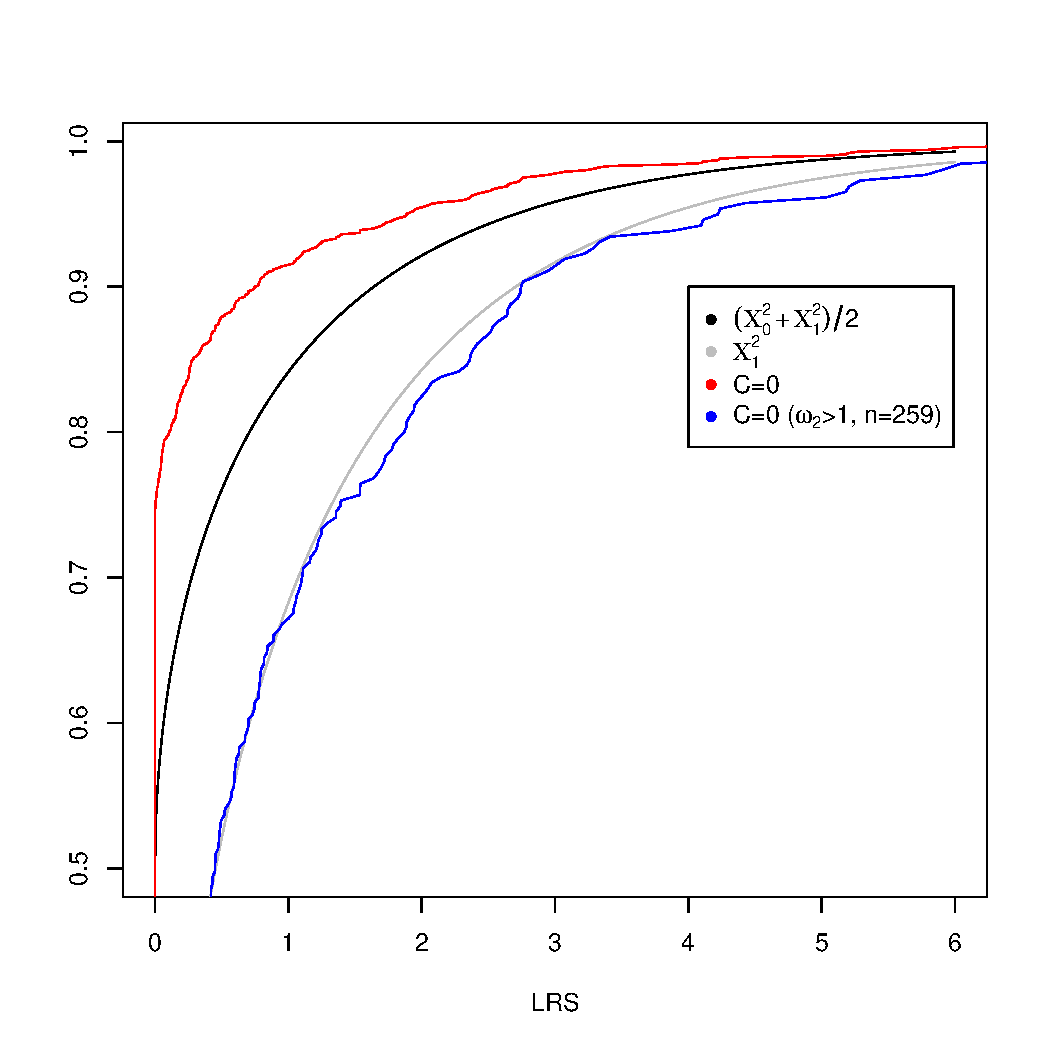
\includegraphics[width=\maxwidth]{figures/data-1} 
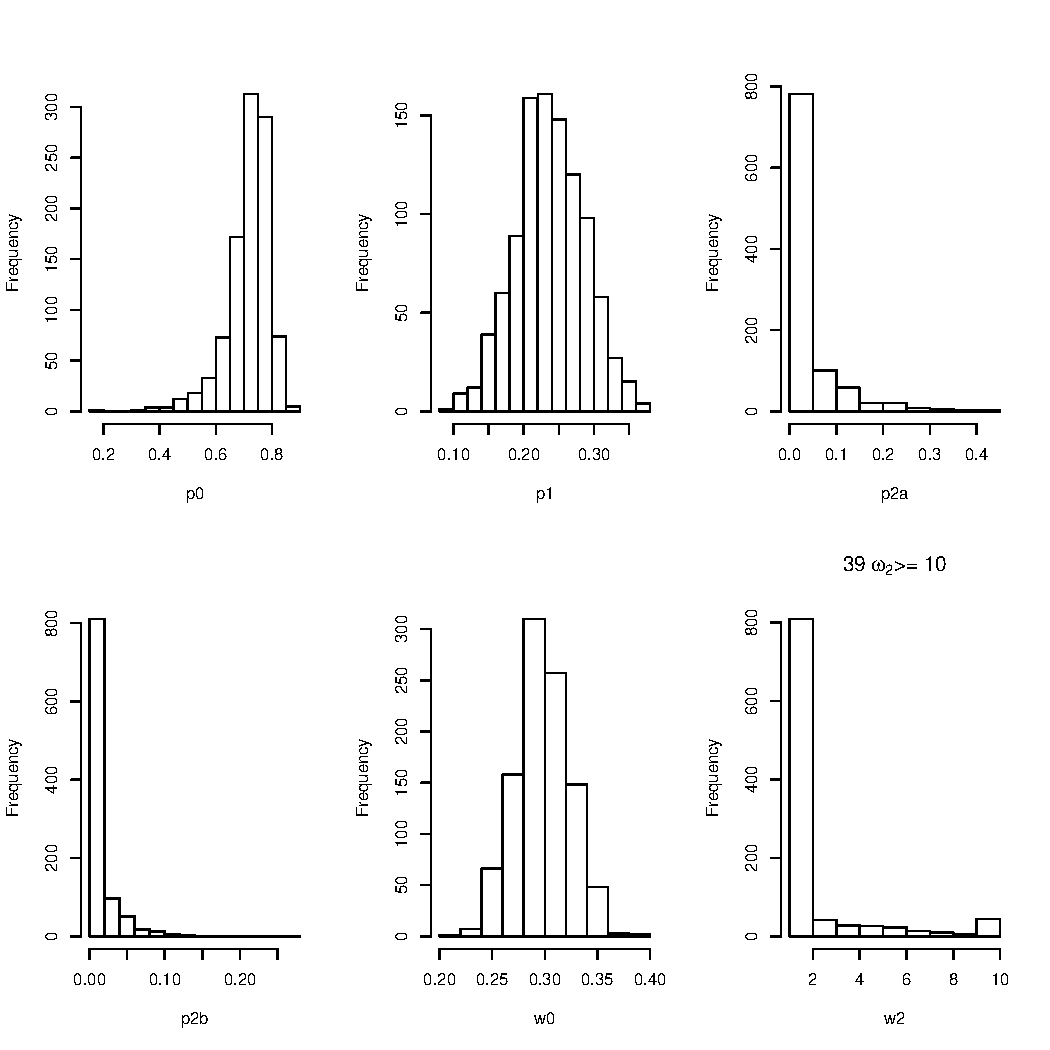
\includegraphics[width=\maxwidth]{figures/data-2} 

}



\end{knitrout}

\clearpage

\begin{lstlisting}
It looks like trouble when p0+p1 is close to 1.

> subset(params,w2>=10)
     p0      p1     p2a     p2b      w0        w2
0.66806 0.32417 0.00523 0.00254 0.29262  11.40713
0.74277 0.25290 0.00323 0.00110 0.29100  63.02795
0.83833 0.15722 0.00375 0.00070 0.34804 663.19371
0.71539 0.27553 0.00656 0.00253 0.28696  45.42719
0.76112 0.23217 0.00514 0.00157 0.29497  28.47234
0.78927 0.20013 0.00845 0.00214 0.32839 998.99965
0.72141 0.27009 0.00619 0.00232 0.28625  90.59841
0.75694 0.23114 0.00913 0.00279 0.32758 159.83998
0.69529 0.28448 0.01436 0.00587 0.30877  11.14156
0.75828 0.23864 0.00235 0.00074 0.32390 999.00000
0.77731 0.21691 0.00452 0.00126 0.30700  42.87754
0.68340 0.30325 0.00925 0.00410 0.27158  12.87590
0.68478 0.30585 0.00647 0.00289 0.27623  80.35478
0.76661 0.22596 0.00574 0.00169 0.27745 998.99969
0.67546 0.31922 0.00361 0.00171 0.27283  11.40887
0.79381 0.19562 0.00848 0.00209 0.31121  14.57206
0.71717 0.27323 0.00695 0.00265 0.24705  15.84686
0.77950 0.21497 0.00433 0.00119 0.33214 692.41967
0.77098 0.21896 0.00783 0.00222 0.30197  13.50125
0.79101 0.20304 0.00474 0.00122 0.29936 672.10568
0.77265 0.20377 0.01866 0.00492 0.31806  10.93935
0.71447 0.27844 0.00510 0.00199 0.29404  14.42786
0.69474 0.29347 0.00829 0.00350 0.27703  18.76982
0.74259 0.23647 0.01589 0.00506 0.30013  64.98670
0.73578 0.25558 0.00641 0.00223 0.29561  36.50829
0.66396 0.32715 0.00595 0.00293 0.28102  17.73306
0.80797 0.17788 0.01160 0.00255 0.31680  11.42403
0.83595 0.15437 0.00817 0.00151 0.31905  15.49704
0.77730 0.21161 0.00872 0.00237 0.29618  42.27299
0.73124 0.26019 0.00632 0.00225 0.31894 998.99969
0.71541 0.28216 0.00174 0.00069 0.29553  52.92020
0.67430 0.31836 0.00498 0.00235 0.25440  21.75579
0.81092 0.18177 0.00597 0.00134 0.32588  13.58634
0.72490 0.26573 0.00686 0.00251 0.28425  25.39505
0.72122 0.27454 0.00307 0.00117 0.25432  35.11208
0.71240 0.26782 0.01438 0.00541 0.29446  12.35679
0.69327 0.29980 0.00484 0.00209 0.29772  14.21954
0.69064 0.30322 0.00426 0.00187 0.25633  31.60063
0.71727 0.27603 0.00484 0.00186 0.25009  10.37322
\end{lstlisting}

\end{document}
